\newpage
\appendix
\chapter{Especificaciones de Cámaras Dahua}
\label{appendix:dahua}

\newpage
\appendix
\chapter{Estructura de un Proyecto Laravel}
La capa de presentación consiste en vistas y controladores que solicitan información a los servicios externos, a los cuales acceden a través de sus APIs.
\clearpage
La estructura de un proyecto de Laravel consiste en:

\vspace{0.5cm}
{\setstretch{1.0}
\dirtree{%
.1 project/.
    .2 \vdots.
    .2 app/.
        .3 \vdots.
        .3 Http/.
            .4 Controllers/.
                .5 CamaraController.php.
                .5 Controller.php.
                .5 LugarController.php.
                .5 \vdots.
            .4 Requests/.
            .4 Kernel.php.
            .4 routes.php.
    .2 config/.
        .3 \vdots.
        .3 app.php.
        .3 database.php.
        .3 compile.php.
    .2 database/.
        .3 \vdots.
        .3 migrations.
    .2 public/. 
        .3 css.
        .3 fonts.
        .3 js.
        .3 \vdots.
    .2 resources/.
        .3 \vdots.
        .3 views.
    .2 vendor/.
    .2 .env.
    .2 \vdots.
    .2 composer.json.
}
}
Donde:

\begin{itemize}
\item \textit{app/} contiene los controladores correspondientes a cada servicio.
\item \textit{config/} contiene la configuración de la aplicación, base de datos, vistas, compilación, etc..
\item \textit{database/} contiene los archivos necesarios para realizar las migraciones de la base de datos, simplificadas con la herramienta Artisan de Laravel \footnote{\url{https://laravel.com/docs/5.3/artisan}}.
\item \textit{public/} contiene las configuraciones de CSS, fuentes y Javascript, además del archivo de la pagina principal index.php.
\item \textit{resources/} contiene las vistas que se presentan al usuario.
\item \textit{vendor/} contiene todos los componentes que incluye Laravel.
\item \textit{.env y composer.json} describen las variables de entorno y las dependencias necesarias para ejecutar la aplicación respectivamente.

\end{itemize}

\newpage
\appendix
\chapter{Diagrama de Paquetes}
A continuación se adjunta un diagrama de paquetes del PFG, como alternativa para representar la distribucion del diagrama de clases.
\begin{landscape}
     \begin{figure}[H]
        \centering
        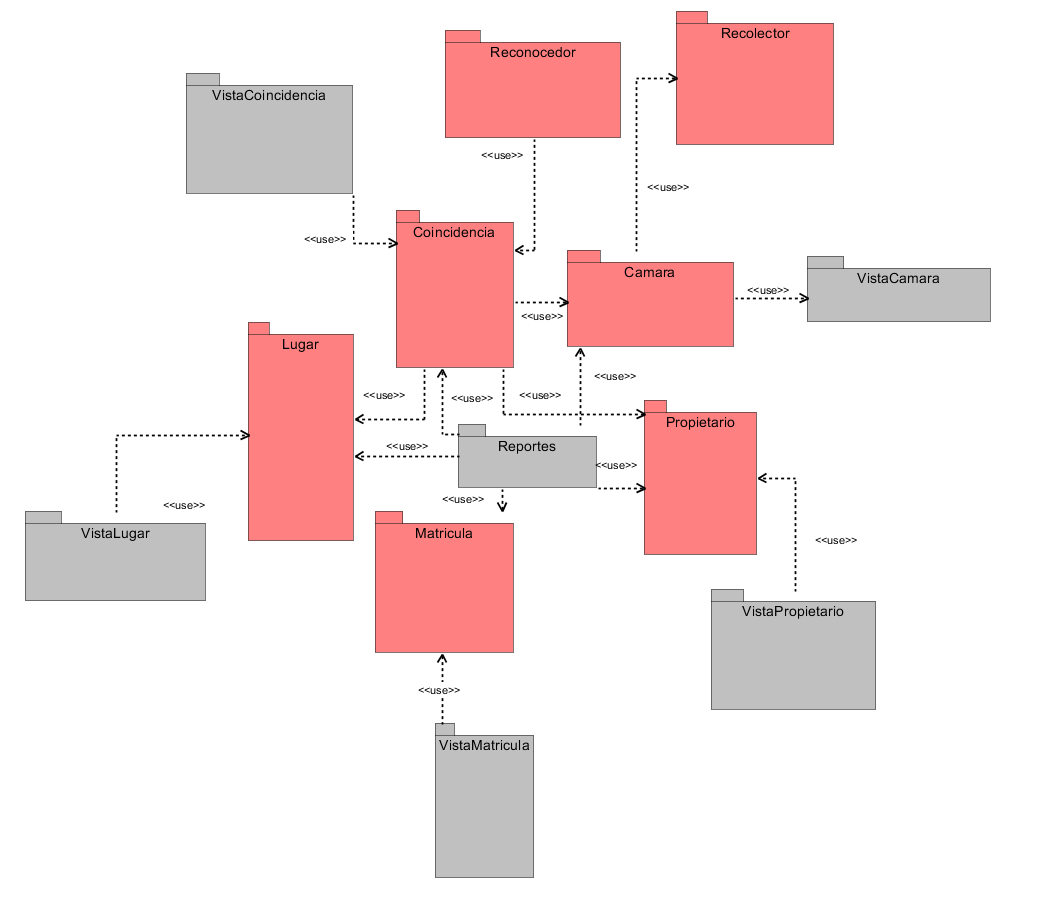
\includegraphics[width=1\textwidth]{class-packages}
        \caption{Modelo Conceptual - Paquetes}
        \label{fig:CLASS-crop}
    \end{figure}
    
        \begin{figure}[H]
        \centering
        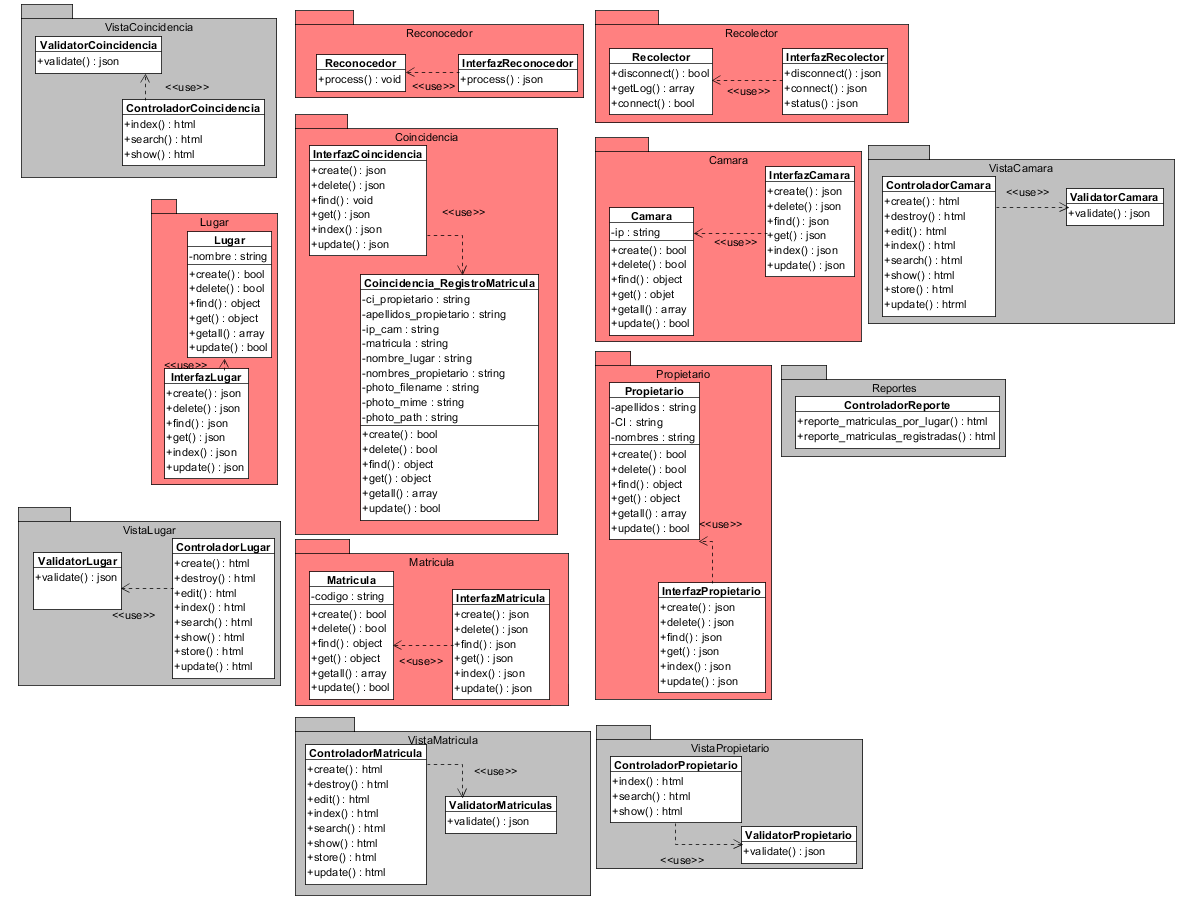
\includegraphics[width=1.1\textwidth]{class-packages-extended}
        \caption{Modelo Conceptual - Detalle}
        \label{fig:CLASS-brief}
    \end{figure}
\end{landscape}